\documentclass[12pt,a4paper]{article}

\usepackage[UTF8]{ctex}
\usepackage{geometry}
\usepackage{graphicx}
\usepackage{booktabs}
\usepackage{hyperref}
\usepackage{setspace}
\usepackage{float}
\usepackage{caption}
\usepackage{array}
\usepackage{longtable}

\geometry{left=2.5cm,right=2.5cm,top=2.5cm,bottom=2.5cm}
\onehalfspacing
\sloppy
\graphicspath{{figures/}}
\hypersetup{colorlinks=true,linkcolor=black,urlcolor=blue,citecolor=black}

\title{从融合到切换：一条澳门路线中的跨文化体验}
\author{UCUG1600 跨文化沟通期末小组报告\\
小组成员（按贡献排序）：待定}
\date{2026年5月8日}

\begin{document}
\renewcommand{\abstractname}{摘要}
\maketitle

\begin{abstract}
澳门常被称为"中西融合"之城。这个标签符合部分现实——中葡双语路牌、葡式建筑和世界遗产街道确实存在——却无法解释我们在一天田野考察中体验到的全部。本报告基于2026年4月澳门田野考察期间收集的照片、视频和路线记录，沿一条从口岸到大三巴牌坊、再到路氹威尼斯人的路线，分析五类城市空间如何将观察者置于不同的文化位置：边境的入境者、商业街的消费者、历史区的观看者、主题娱乐的参与者和巴士上的乘客。报告提出"文化角色切换"的概念，论证澳门的跨文化特征并非固定在某一地点，而是随着路线移动不断转变。这一发现对"中西融合"的单一标签提出了补充，指出空间移动本身是跨文化理解的重要组成部分。
\end{abstract}

\section{引言}

在澳门口岸我们最先注意到的是声音。扶梯嗡嗡作响，广播用三种语言回荡，几百号人在队伍里挪步，没什么人说话。没人在看什么遗产建筑。他们在读头顶的指示牌，攥着证件，琢磨该排哪条队。这也是澳门，尽管没有旅游手册会提到它。

澳门被贴上"中西融合"的标签，这标签并非全错。联合国教科文组织收录的"澳门历史城区"确实展现了中西之间在建筑、宗教和城市技术方面的长期交流（UNESCO World Heritage Centre, n.d.）。中葡双语路名和天主教教堂立面真实可见。麻烦在于，"融合"暗示某种已经调和好的东西，而我们在地面上感受到的却一直在变。大三巴牌坊附近，小吃摊和纪念品人潮在我们还没走到石立面之前就把我们拉进了消费。在路氹，威尼斯人画出来的天幕和NBA投篮游戏把欧洲意象和美国体育折叠进了同一条购物动线。站点之间的巴士上，城市一帧一帧地闪过车窗。

本报告问一个直接的问题：澳门的城市空间如何改变观察者在移动过程中做了什么、注意到什么？我们用"文化角色切换"来描述不同空间如何将观察者置于不同位置——边境的入境者、美食街的消费者、历史区的观看者、路氹的参与者、巴士上的乘客。这些切换与课程中自我与他者、文化敏感性、言语与非言语沟通等主题相连。我们让田野材料来引导分析，根据实际观察来处理每个地点，而不是套用一个预设概念。

分析局限于一次田野考察路线上的公共空间。我们没有做访谈，因此不代表澳门居民、游客或工人的立场。以下内容先介绍概念和方法，再沿路线走过五类空间，最后讨论这种方法对理解澳门跨文化沟通有什么帮助。

\section{概念框架与文献综述}

本报告借鉴四个领域的文献：路线与被定位的观察者、旅游与被营造的体验、语言景观与非言语沟通、以及澳门自身的遗产和语言政治。这四个领域为我们提供了阅读田野材料的工具，而不用把概念硬套到每一个地点上。

\subsection{空间、路线与被定位的观察者}

城市空间塑造了人们如何进入、观看、停留和感知一个地方。Lefebvre（1991）的空间生产理论将空间视为由社会关系、制度安排和日常实践所构成的东西。在我们的澳门路线上，口岸走廊、遗产台阶和巴士车厢各自以不同方式安排了人们的移动。de Certeau（1984）将步行视为人们使用和诠释城市的日常实践。对我们来说，路线本身就是分析的一部分。澳门的文化差异恰恰在空间转换之间变得可见。

Pink（2009）的感官民族志工作指向同样的方向。只依赖图片的田野观察会遗漏很多。人群密度、噪音、移动速度、身体的疲惫感——这些都在塑造我们注意到的东西。一些最敏锐的观察发生在转换中，即一个空间和下一个空间之间的时刻，而不是在计划停留的站点。把这些时刻包括进来，让本报告不至于变成一张旅游景点的清单。

\subsection{旅游、本真性与被营造的体验}

旅游空间往往预先决定了游客看到什么、怎么拍照。MacCannell（1973）的"被营造的本真性"概念解释了旅游场景如何为游客安排一个"真实"的版本来消费。Wang（1999）将本真性推得更远：即使一个物件在历史上并非原物，参与的感觉仍然可以产生一种切身经历的体验。Urry和Larsen（2011）的"游客凝视"表明，游客的观看方式受到景点、拍照位置和社会期望的塑造；Edensor（2000）则指出，拍照、购物和排队是游客完成旅游空间的方式之一。

这些想法有助于区分大三巴牌坊和威尼斯人。两者都使用欧洲符号，都吸引拍照，但观看方式不同。大三巴牌坊依靠历史遗存和世界遗产地位；威尼斯人依靠复制的立面、室内天幕和为沉浸感设计的零售街道。一个是遗产观看，一个是沉浸式消费。澳门不寻常之处在于两者可以在同一条路线上、一个下午内接连出现。

\subsection{语言景观与非言语沟通}

跨文化沟通也发生在对话之外。Landry和Bourhis（1997）将语言景观定义为语言在公共空间中的可见性：路名、招牌、广告、店面。Scollon和Scollon（2003）的地理符号学要求我们通过标牌所处的位置、朝向和材质来阅读它，而不仅仅是上面的文字。在澳门，中葡双语路牌、酒店导视系统和NBA产品标签都属于值得阅读的公共标牌。

非言语沟通贯穿同样的空间。Hall（1959）将空间本身描述为一种无声的语言——这个想法契合口岸的排队队伍、教堂内部的安静，以及投篮游戏的喧闹。UCUG1600课程同时强调言语和非言语沟通。澳门是一个好案例：部分文化信息写在标牌上，其余的由移动、灯光和拥挤来传递。

\subsection{澳门研究与课程视角}

澳门研究将这些更广泛的理论带回到一个具体的地方。Chung（2009）将澳门的遗产保护与城市发展和身份叙事联系起来。Chu（2015）研究澳门的奇观城市空间，展示路氹酒店如何通过视觉尺度和主题建筑重塑城市想象。Yan（2019）考察澳门公共空间中的语言选择并将其与身份和权力联系起来。Ma和Mu（2023）表明澳门的多语标牌根据场所功能和目标读者来安排。

这些研究呈现出一个清晰的模式："中西融合"描述了澳门的一部分，但不是全部。一个更有用的问题是不同空间如何安排观察者与文化符号之间的关系——这个问题与课程中自我与他者、文化敏感性、跨文化叙事等主题相连。我们追问的是空间在各自场景中如何运作，而不是判断它们是"真的"还是"假的"。

\section{研究方法}

\subsection{田野地点与路线}

材料来自2026年4月课程田野考察期间的澳门之行。小组以学生和游客的双重身份进入澳门公共空间。路线大致为：口岸与出入境空间 $\rightarrow$ 口外交通区域与道路景观 $\rightarrow$ 历史商业街道 $\rightarrow$ 大三巴牌坊、教堂空间、圣物艺术空间与大炮台 $\rightarrow$ 巴士与道路过渡 $\rightarrow$ 路氹酒店综合体、威尼斯人及NBA主题空间 $\rightarrow$ 回程交通。交通空间被纳入发现部分，因为移动不断改变着观察者的位置。它们不是目的地之间的空白时间。

\subsection{数据收集方法}

小组记录了人群、移动路线、标牌、建筑和互动实践。照片和视频保存了口岸指示牌、商业街人群、双语路牌、威尼斯人天幕、NBA投篮区域和车窗景观等场景。路线本身也被视为材料，因为它展示了一个地方如何转变为另一个地方。田野笔记还记录了声音水平、光线条件和身体疲惫感。整理材料后，小组约有69个逻辑媒体条目，包括照片、视频和从视频中提取的选定帧。报告中选取的图像是因为它们支持论证且未突出可识别的个人。

\subsection{范围、伦理与AI使用}

田野考察未包含正式访谈，因此报告不能代表澳门居民、游客、店主或工人的主观观点。分析局限于公共空间中可观察的要素：语言、建筑、声音、移动路线、人群和消费标牌。当图像包含人群时，仅作为公共空间使用方式的证据，如游客观看或交通密度。报告不分析可识别的个人。

生成式AI在早期阶段辅助了主题探索和关键词建议。小组选定研究问题、选择材料并构建论证。所有田野观察均来自实际行程。

\section{发现}

本节按田野考察路线的顺序展开。商业街道在历史区域之前讨论，因为根据我们的体验，游客通常先经过小吃摊和人潮才到达大三巴牌坊。交通被单独处理，因为巴士和桥梁改变了观察的角度，使不同版本的澳门在运动中显现。

\subsection{边境澳门}

那天我们遇见的第一个澳门由扶梯、指示牌和交通接驳组成。没有人从出入境大厅看到大三巴牌坊。在正式进入城市之前，我们已经在读标牌、跟着人群、切换交通方式。跨文化体验从这里就开始了，但它开始于被管理的移动。

\begin{figure}[H]
  \centering
  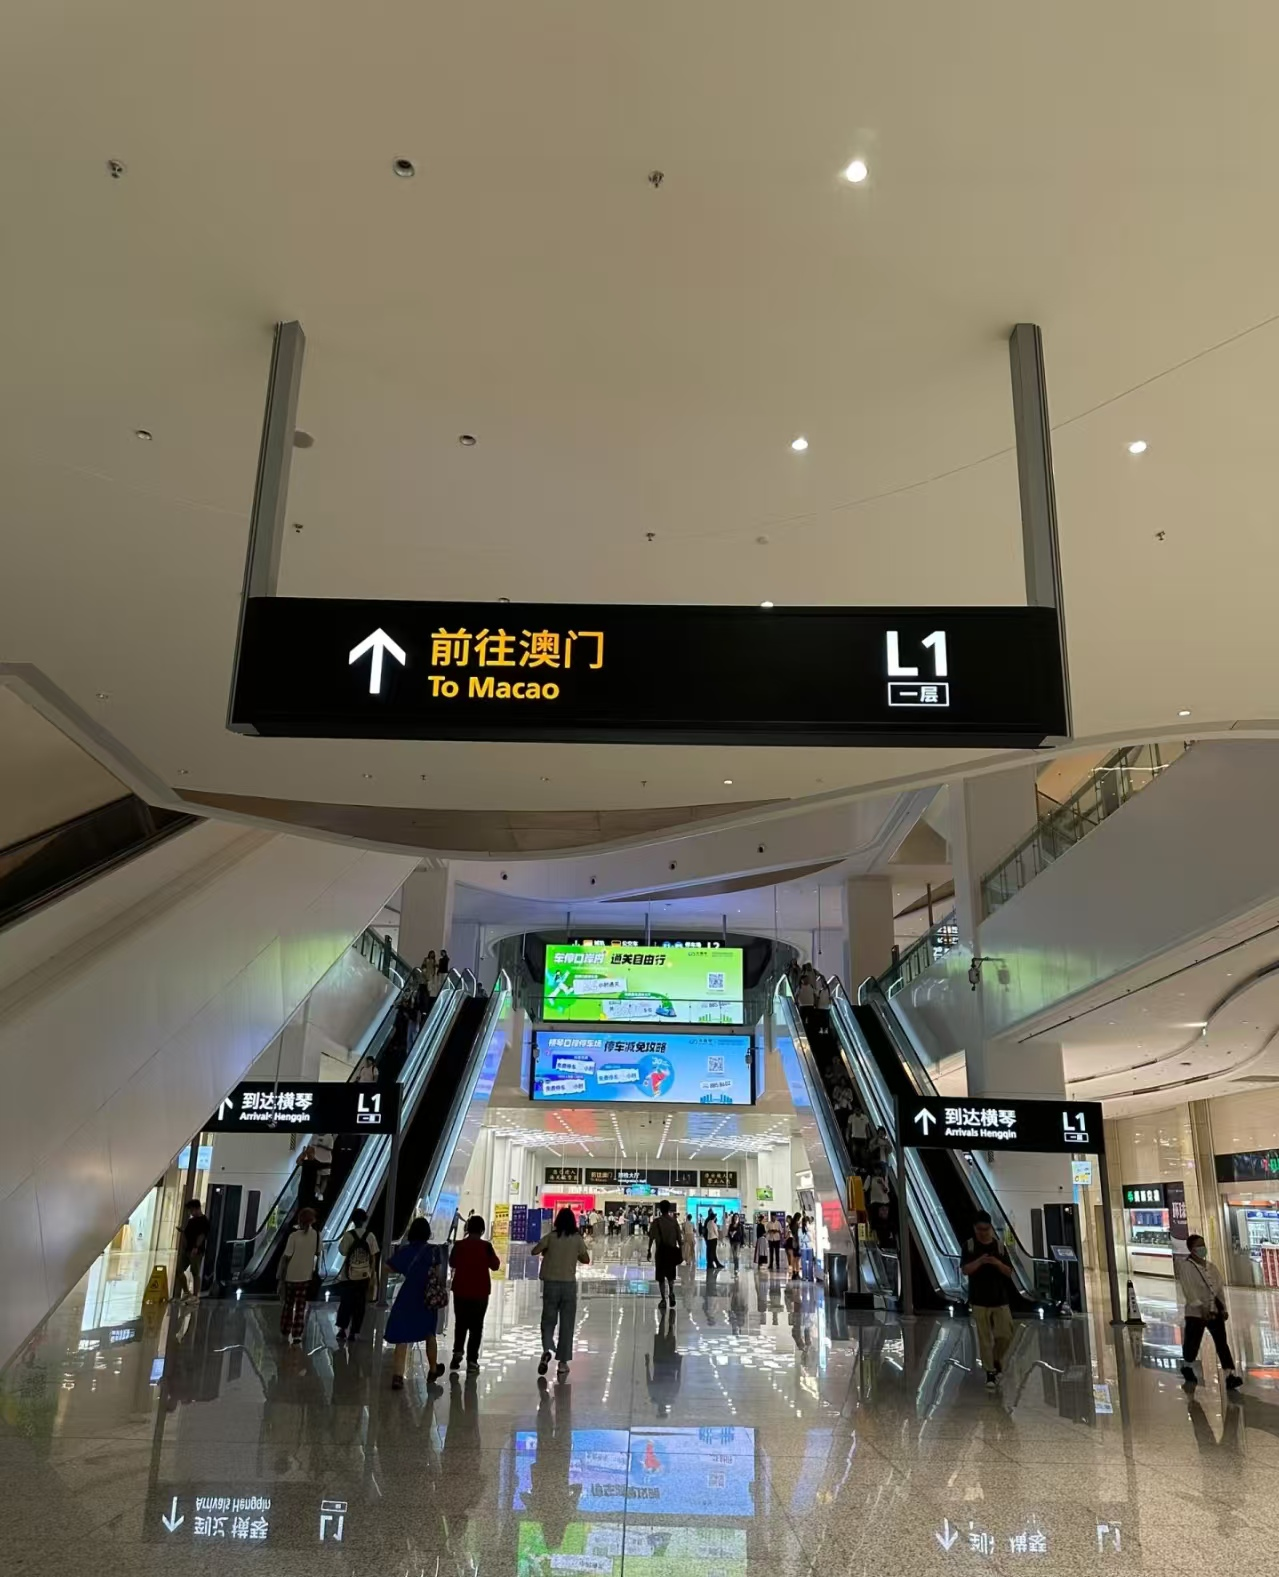
\includegraphics[width=0.82\linewidth]{fig01_border_sign.jpg}
  \caption{前往澳门途中的交通与导视空间。指示牌、扶梯和交通节点出现在旅游景点之前，首先设定了身体的移动方向。}
\end{figure}

边境的沟通并不依赖面对面对话。指示牌、扶梯和走廊告诉人们往哪里走。Hall（1959）将空间视为无声语言的看法在这里很贴切：规则很少被详细解释，但身体仍然沿着特定路径移动，没有人提问。澳门在这个阶段不像一个供人观看的文化场景，更像一个需要通过的系统。

\subsection{商业街道}

离开口岸和交通空间后，路线进入了大三巴牌坊附近的商业街道。这不是什么安静的历史入口。小吃摊先冲过来。蛋挞和牛肉干的气味飘在石立面之前。纪念品商店、密集的招牌和多语种店名把游客拉进一个旅游版的澳门，而遗产景点还没有出现。

\begin{figure}[H]
  \centering
  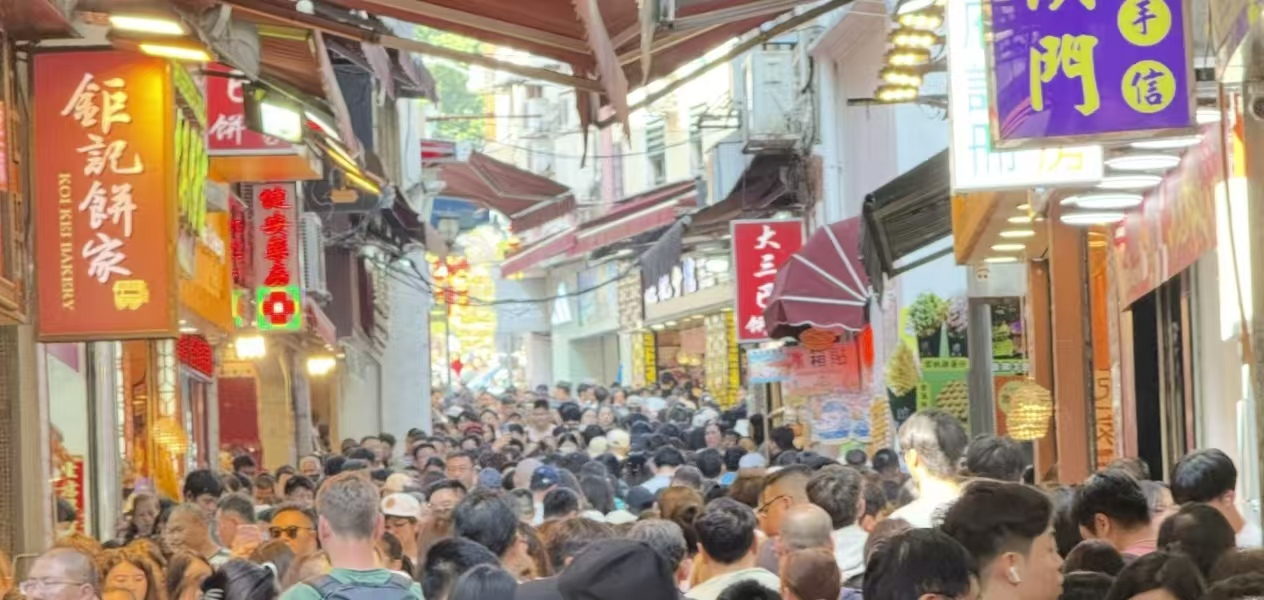
\includegraphics[width=0.82\linewidth]{fig02_commercial_crowd.jpg}
  \caption{大三巴牌坊附近商业街的密集人群。通往遗产地标的路线首先经过商铺、标牌和拥挤的游客移动。}
\end{figure}

商业街上的语言有明确的分工。中文承载着店主和顾客之间日常的商业交谈。英文帮助游客辨认商品和服务。葡萄牙文通常在标牌上更小，但以视觉方式标记着澳门的历史身份。Landry和Bourhis（1997）提醒我们，公共空间中可见的语言塑造着人们对地方身份的理解。在这些街道上，多语标牌与产品陈列和试吃摊位协同工作，而非孤立存在。

\begin{figure}[H]
  \centering
  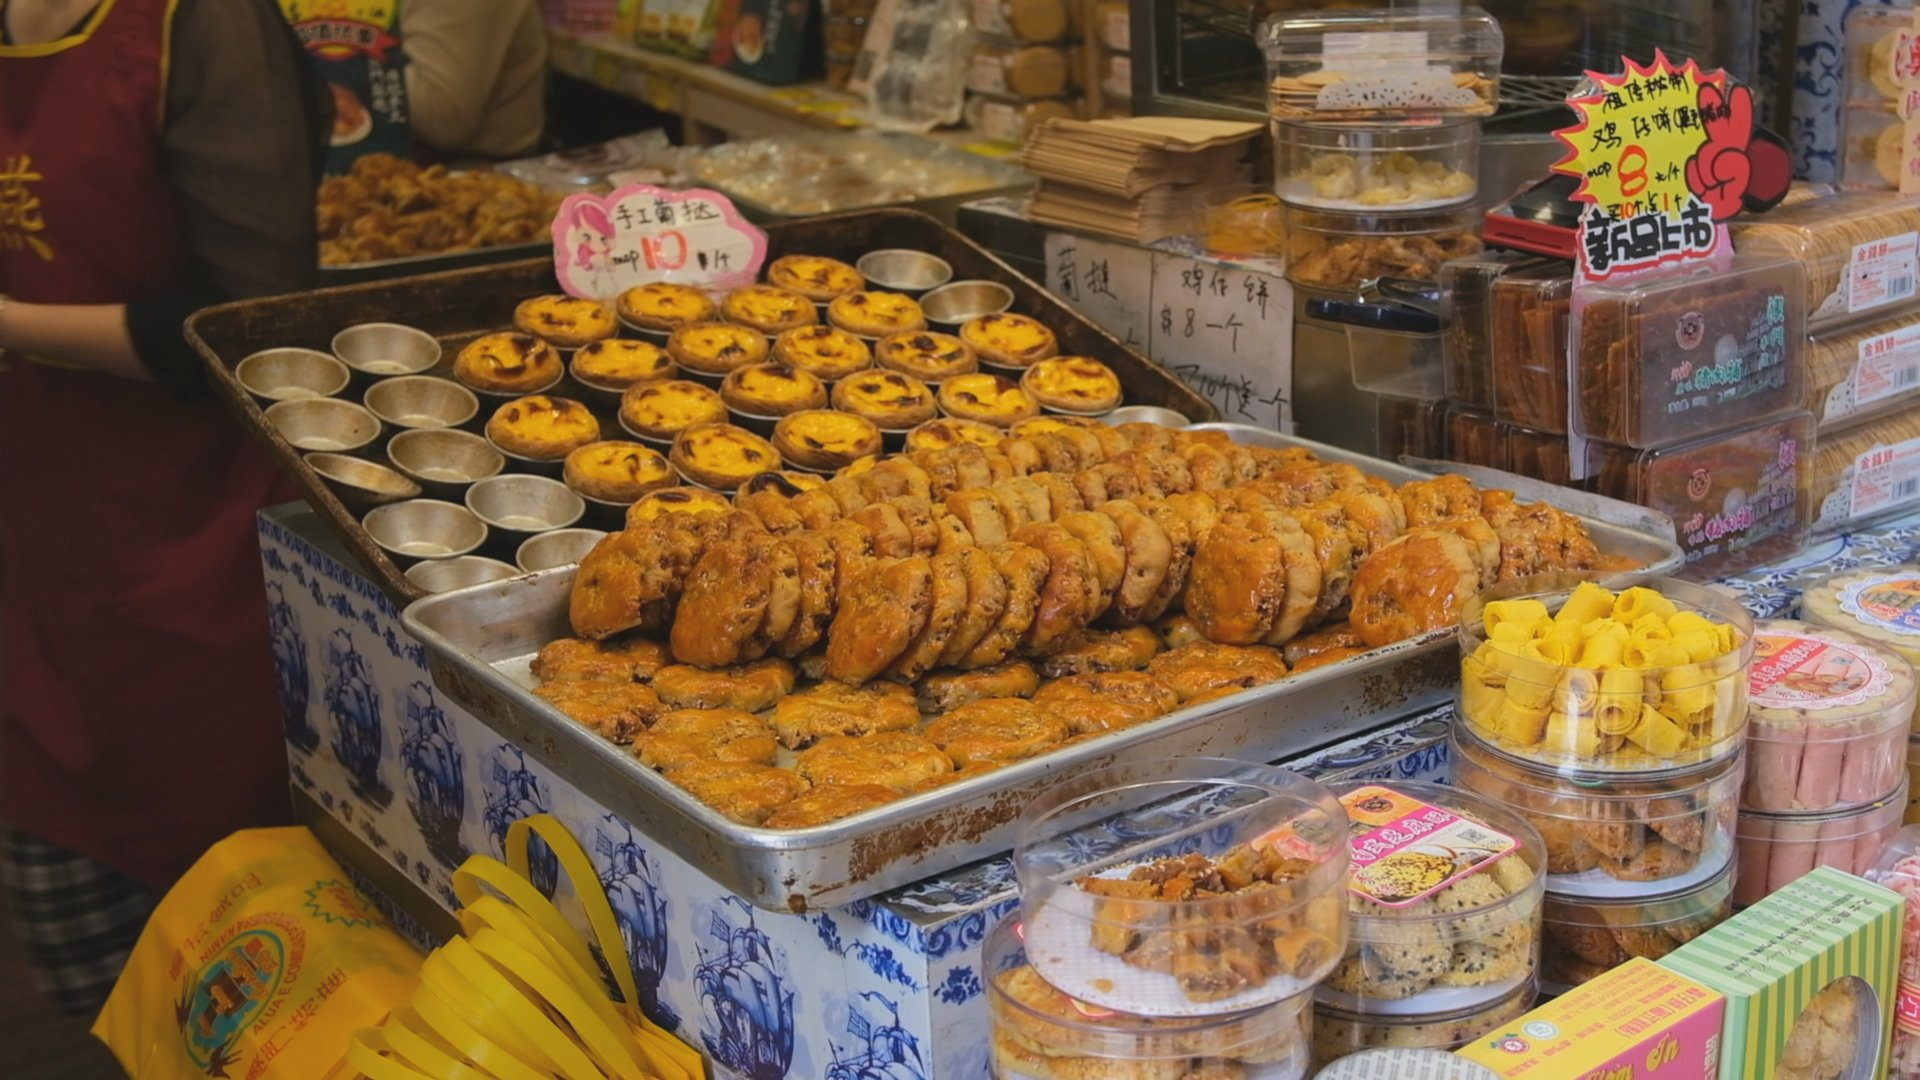
\includegraphics[width=0.82\linewidth]{fig03_food_street.png}
  \caption{街边烘焙店与小吃摊。品尝、购买和短暂停留让游客通过身体和感官进入商业化历史街区。}
\end{figure}

在这个街道空间里，观察者最清晰的角色是消费者。人们看标牌、买小吃、跟着人流走向大三巴牌坊。商业把遗产地标包装成了一个容易进入、难以跳过的旅游体验。对我们来说，澳门的历史先通过味道和人潮到达，比任何教科书版本都早。

\subsection{历史澳门}

过了商业街，节奏变了。大三巴牌坊、教堂空间和大炮台周围的历史区域需要一种不同的注意力。你得慢下来，抬头看立面，读路牌，穿过坡道和石墙。历史就在那里，但你得走进去。

\begin{figure}[H]
  \centering
  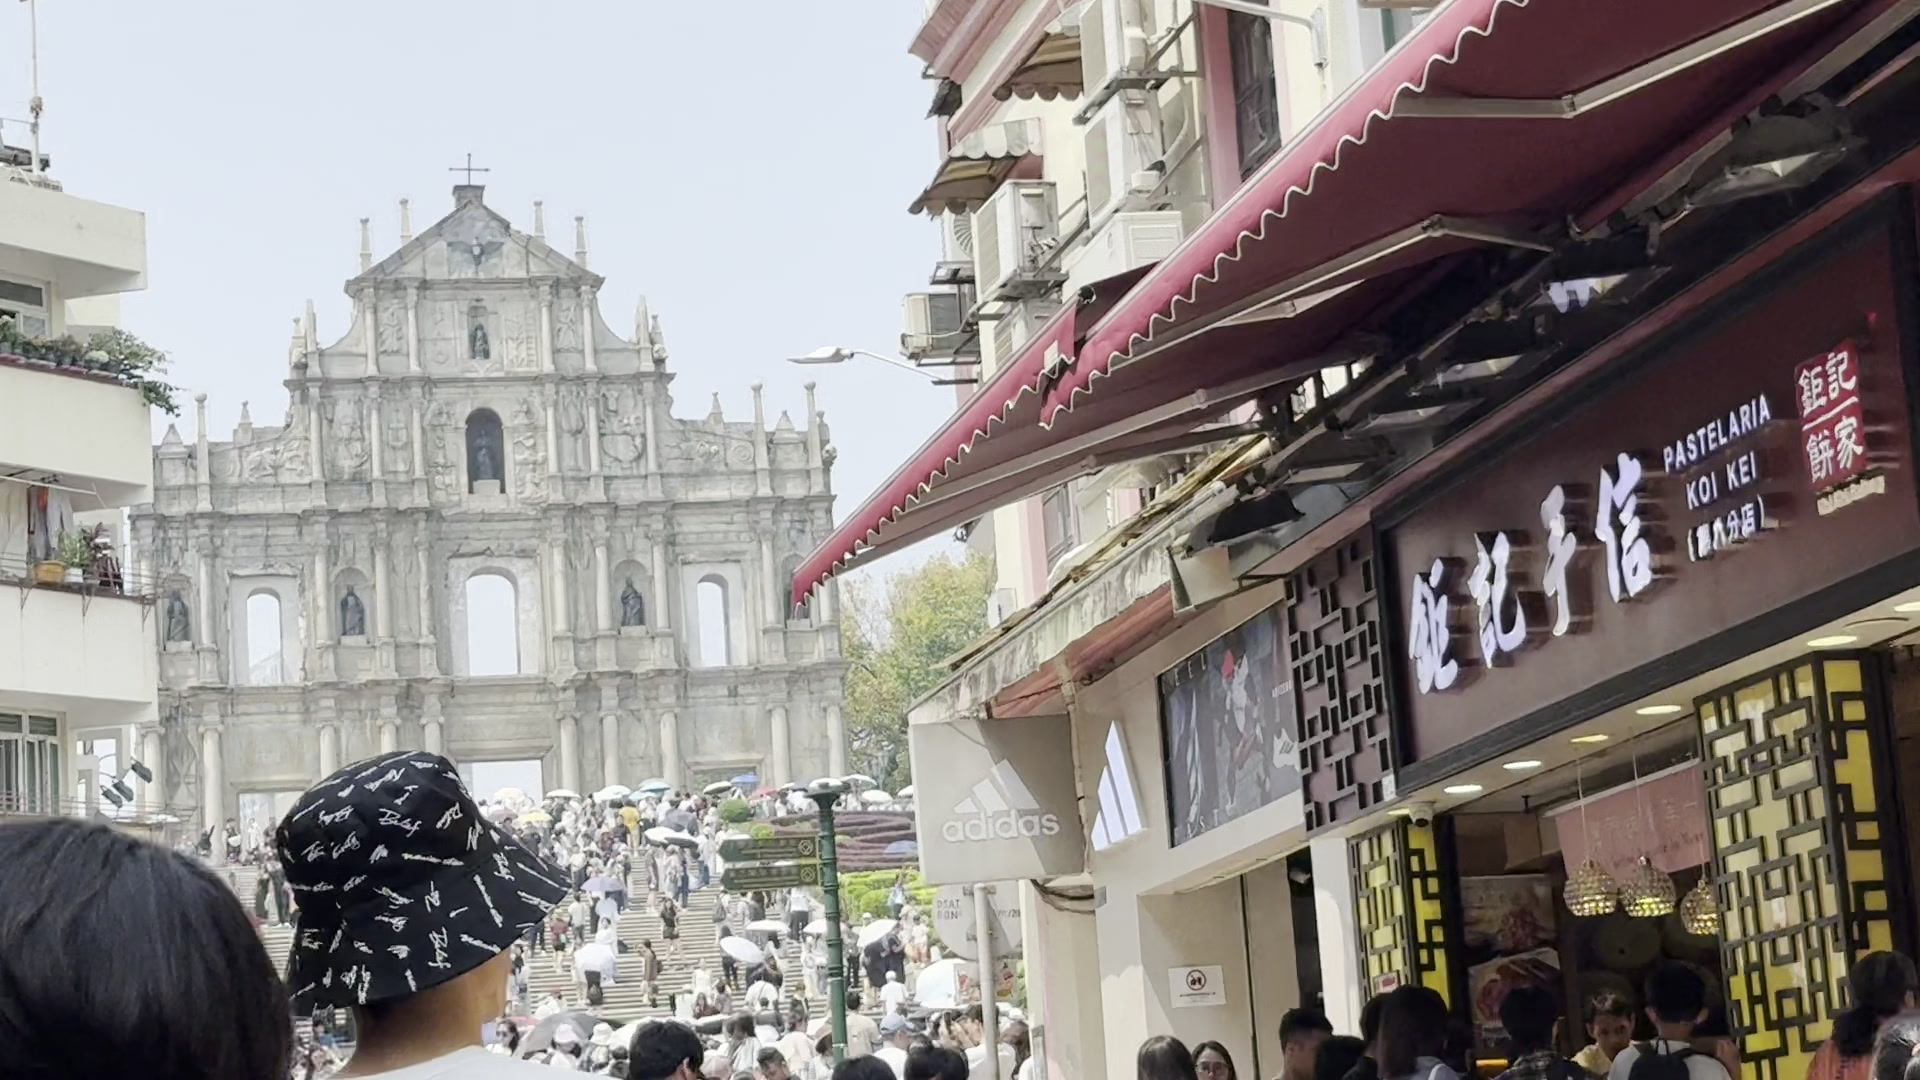
\includegraphics[width=0.82\linewidth]{fig11_street_to_ruins.jpg}
  \caption{通向大三巴牌坊的街景。立面并非突然出现，而是由商铺标牌、人群和街道坡度逐渐引出。}
\end{figure}

大三巴牌坊是澳门最具辨识度的遗产标志之一。游客走向立面，在广场停步，抬头拍照。台阶和广场让正面观看变得容易。MacCannell（1973）的被营造本真性有助于解释正在发生的事：遗产留在原处，但广场、台阶和拍照位置也为游客做了安排。石头有四百年了。摆拍是现在。

双语路牌提供了另一种阅读历史的方式。一个标牌引导移动，但它也将中文、葡文、历史命名和街景放在了同一个表面上。Scollon和Scollon（2003）主张标牌应该在其具体位置中被阅读。澳门的蓝白瓷砖路牌之所以重要，是因为它们结合了两种语言，嵌在老建筑、小巷和旅游路线之中。一个地点，多于一重历史体系。

\begin{figure}[H]
  \centering
  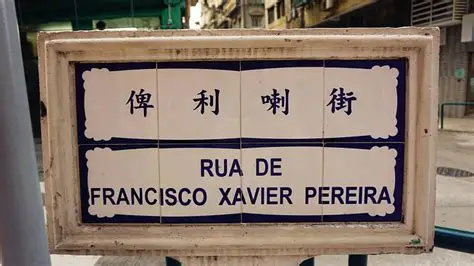
\includegraphics[width=0.72\linewidth]{fig05_bilingual_tile_street.png}
  \caption{``俾利喇街''的蓝白瓷砖路牌。葡文历史名称与中文街名出现在同一标牌上，将路名变成了日常的历史文本。}
\end{figure}

\begin{figure}[H]
  \centering
  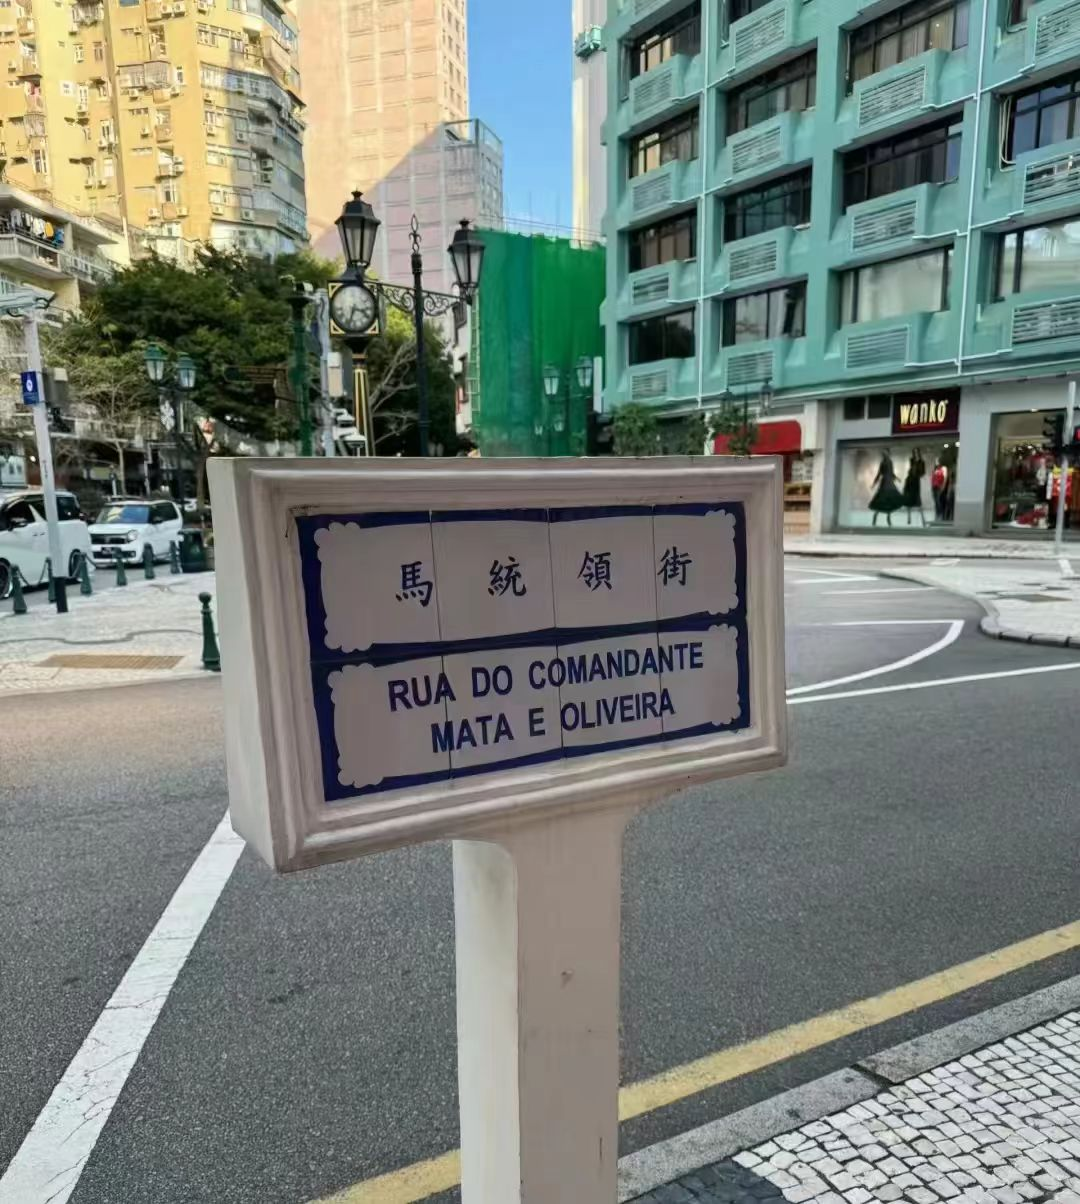
\includegraphics[width=0.72\linewidth]{fig06_bilingual_street_sign.jpg}
  \caption{``馬統領街''路牌。中葡文名称在街道中保留了不止一层城市记忆。}
\end{figure}

大炮台和周围的坡道使这种身体维度更加清晰。沿坡道走向观景台，经过石墙，穿过窄门，历史从一个视觉对象变成了一个身体对象。站在观景台上俯瞰现代城市，观察者从一个与过去相连的位置观看今天的澳门。历史区域把我们从消费者的角色推离，推向了观看者和阅读者的角色。

\begin{figure}[H]
  \centering
  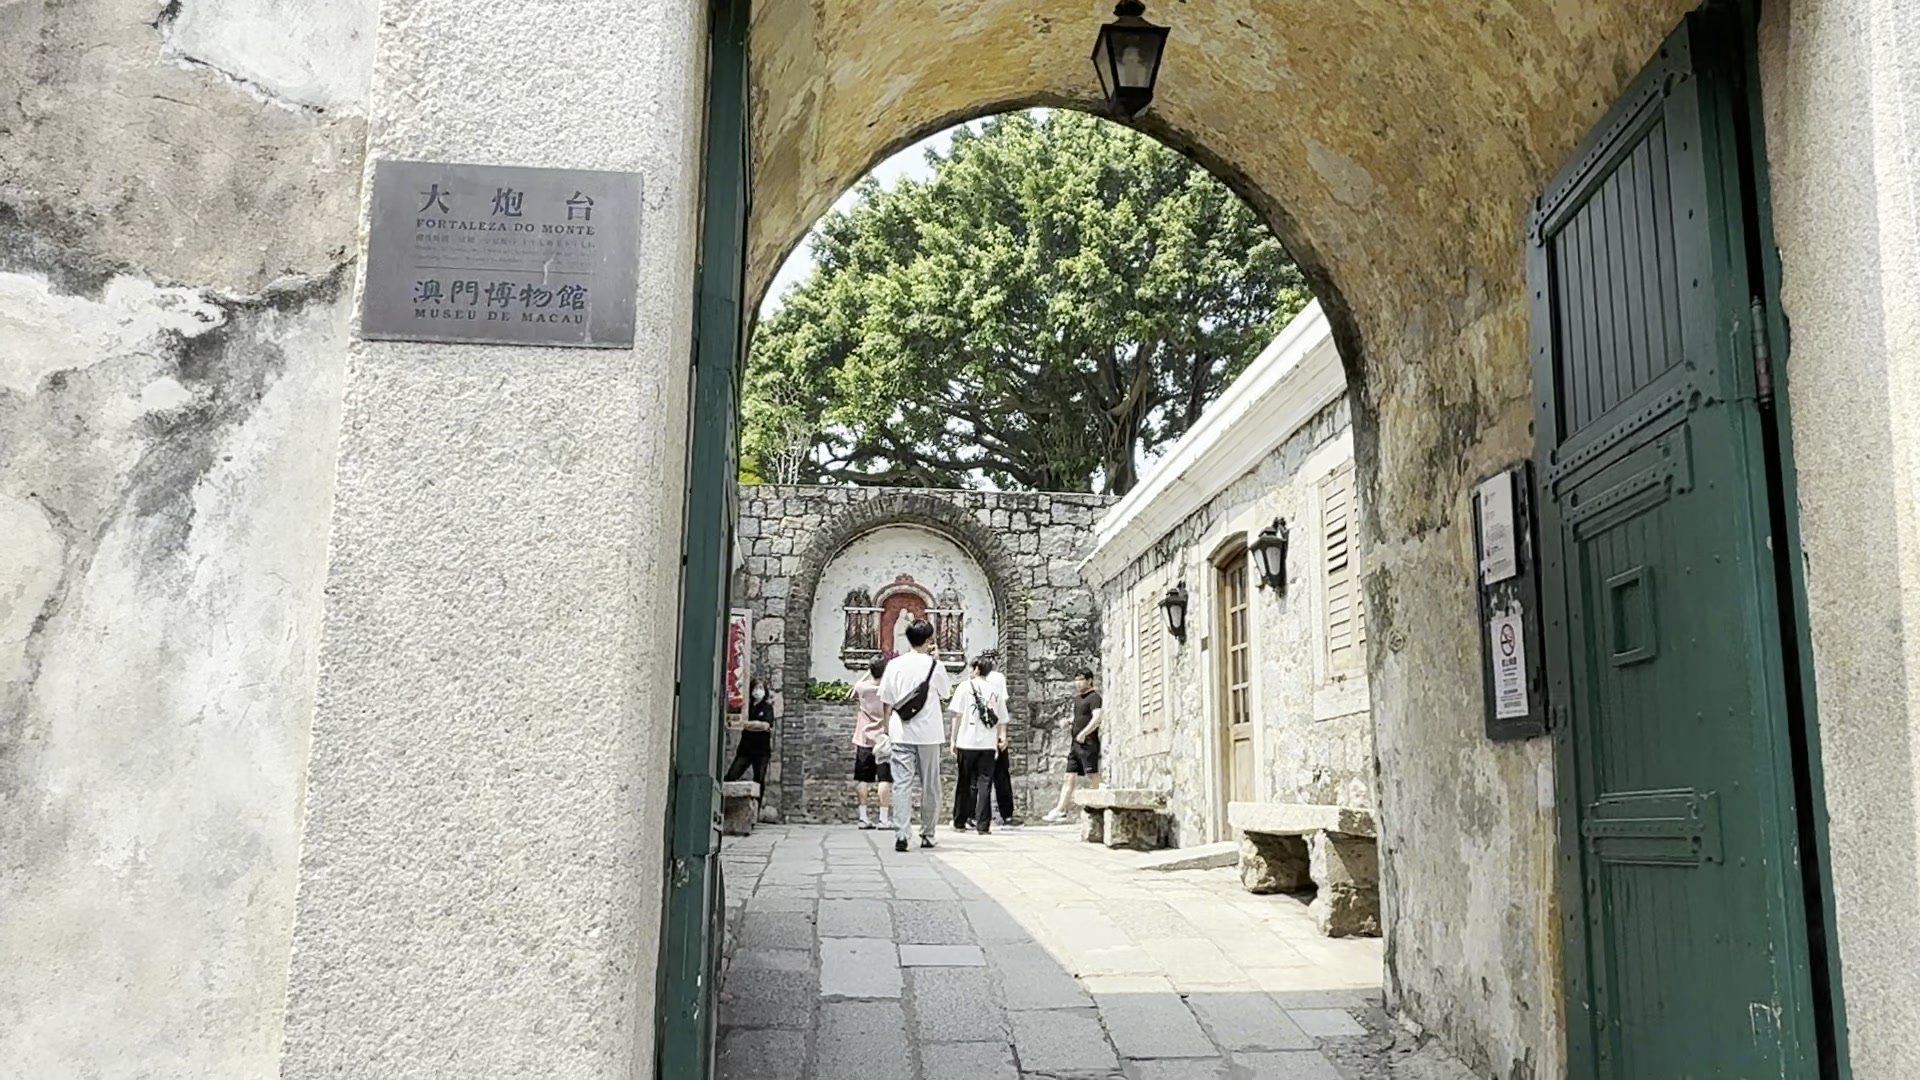
\includegraphics[width=0.82\linewidth]{fig12_fort_gate_path.jpg}
  \caption{通往大炮台的石门与路径。坡道、石墙和入口要求游客穿行于遗产之中，而非仅仅从远处观看。}
\end{figure}

\subsection{奇观澳门}

到达路氹后，文化体系又转了。酒店群、威尼斯人、巴黎人和NBA主题空间并不讲述一段中葡历史。它们把欧洲地标、赌场酒店和体育品牌放进了一条消费路线。这里的跨文化沟通更接近全球娱乐，而非本地遗产。

\begin{figure}[H]
  \centering
  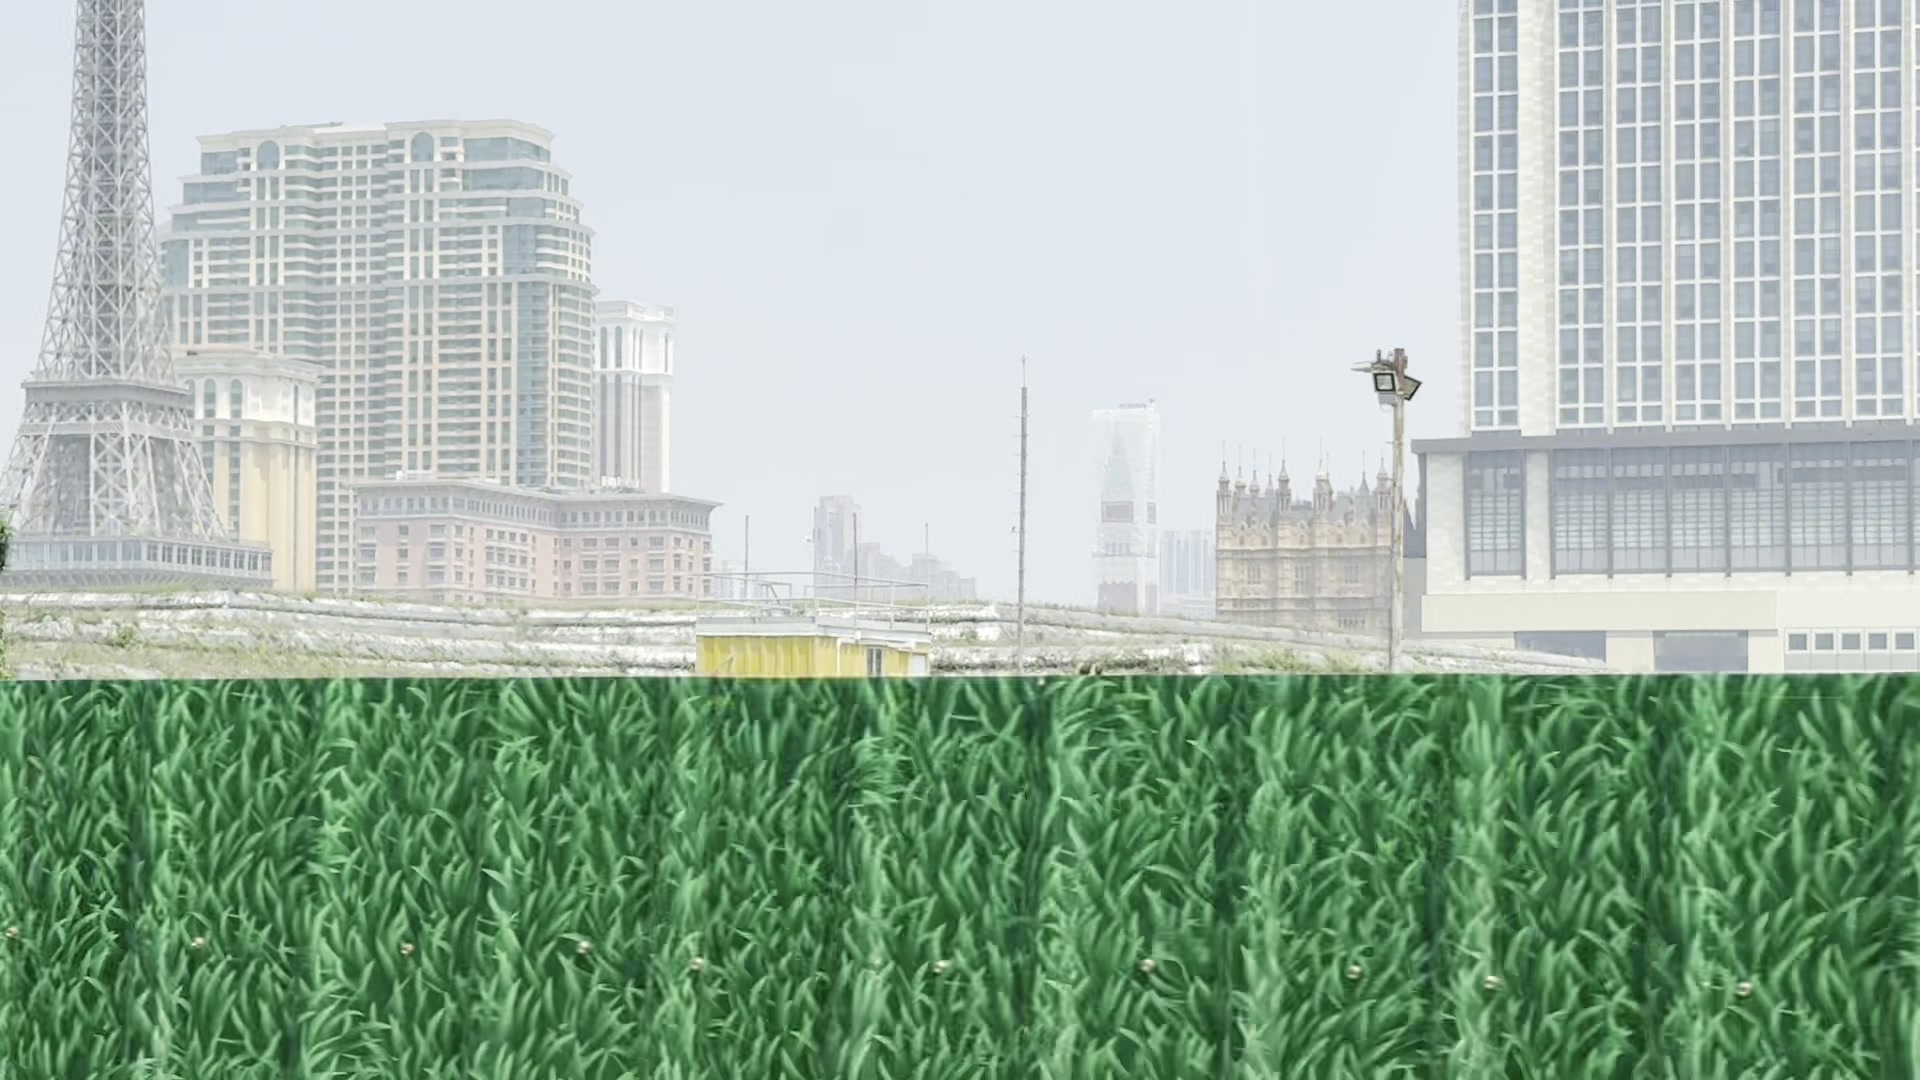
\includegraphics[width=0.82\linewidth]{fig07_cotai_parisian_window.jpg}
  \caption{车窗中看到的路氹酒店群与主题建筑。复制的地标、酒店和道路在移动视野中一同出现。}
\end{figure}

威尼斯人是澳门内部一个被设计出来的欧洲想象。画成天空的室内天花板、壁画和古典风格装饰创造了一个用于购物、拍照和逗留的环境。叫它"假欧洲"会错过重点。它的来源和大三巴不同：一个依托历史层积和遗产叙事，另一个依托刻意设计和沉浸感。两者都生产体验，但材料不同。

\begin{figure}[H]
  \centering
  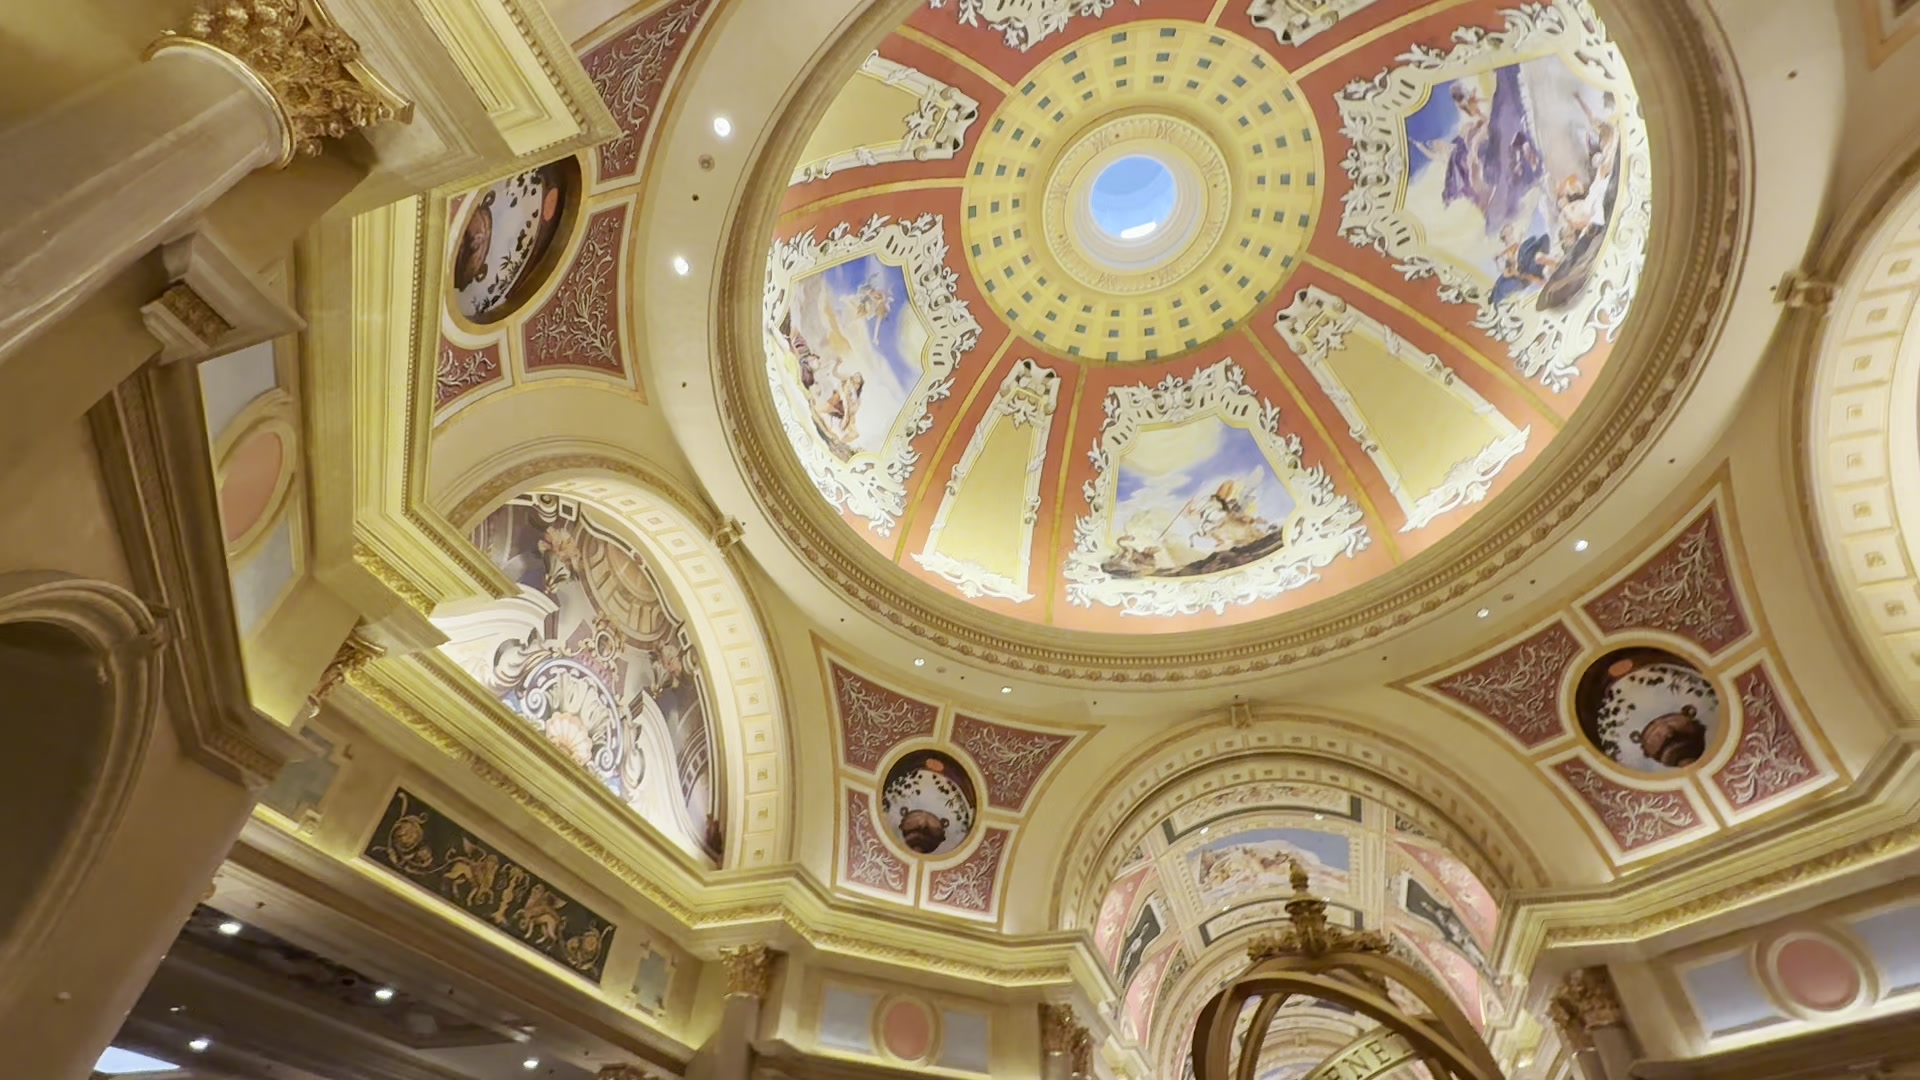
\includegraphics[width=0.82\linewidth]{fig8_venetian_dome.jpg}
  \caption{威尼斯人室内穹顶。向上观看、壁画和古典风格装饰将欧洲想象安置在购物综合体内部。}
\end{figure}

导视系统也很重要。路氹综合体更像一条消费路线而非单一景点。赌场、酒店、餐厅和主题建筑通过同一套导视系统相连。这些标牌告诉游客往哪里走，也引导身体走向下一个消费场景。

\begin{figure}[H]
  \centering
  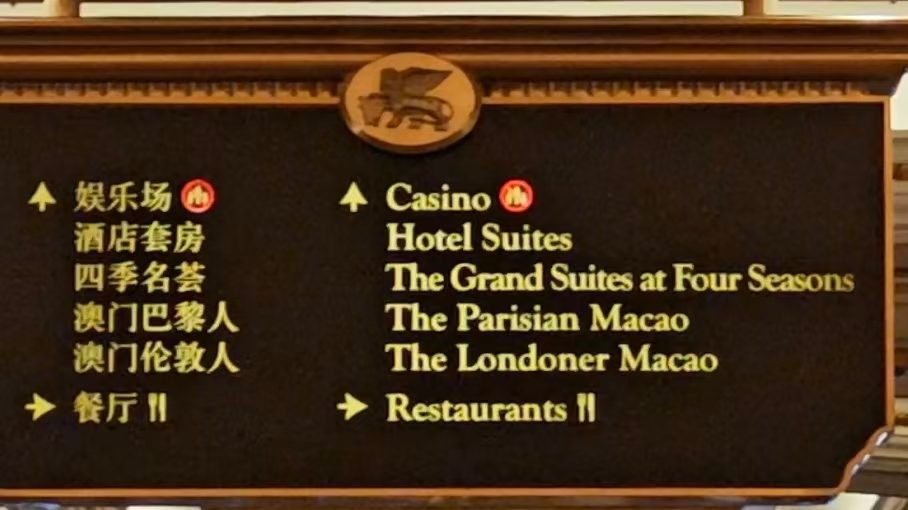
\includegraphics[width=0.82\linewidth]{fig08_wayfinding_casino.jpg}
  \caption{赌场与酒店导视。住宿、博彩、餐饮和购物由一套导视系统串联。}
\end{figure}

NBA主题空间把全球流行文化变成了游客可以触摸和玩耍的东西。美国体育文化不是通过文字展板来讲解的，它通过货架上的球衣、球场设计、投篮动作和计分屏幕进入身体。Wang（1999）关于存在本真性的讨论恰好适用：游客可能并不了解美国篮球的全部历史，但当球穿过篮筐的那一刻，参与感是真实的。

\begin{figure}[H]
  \centering
  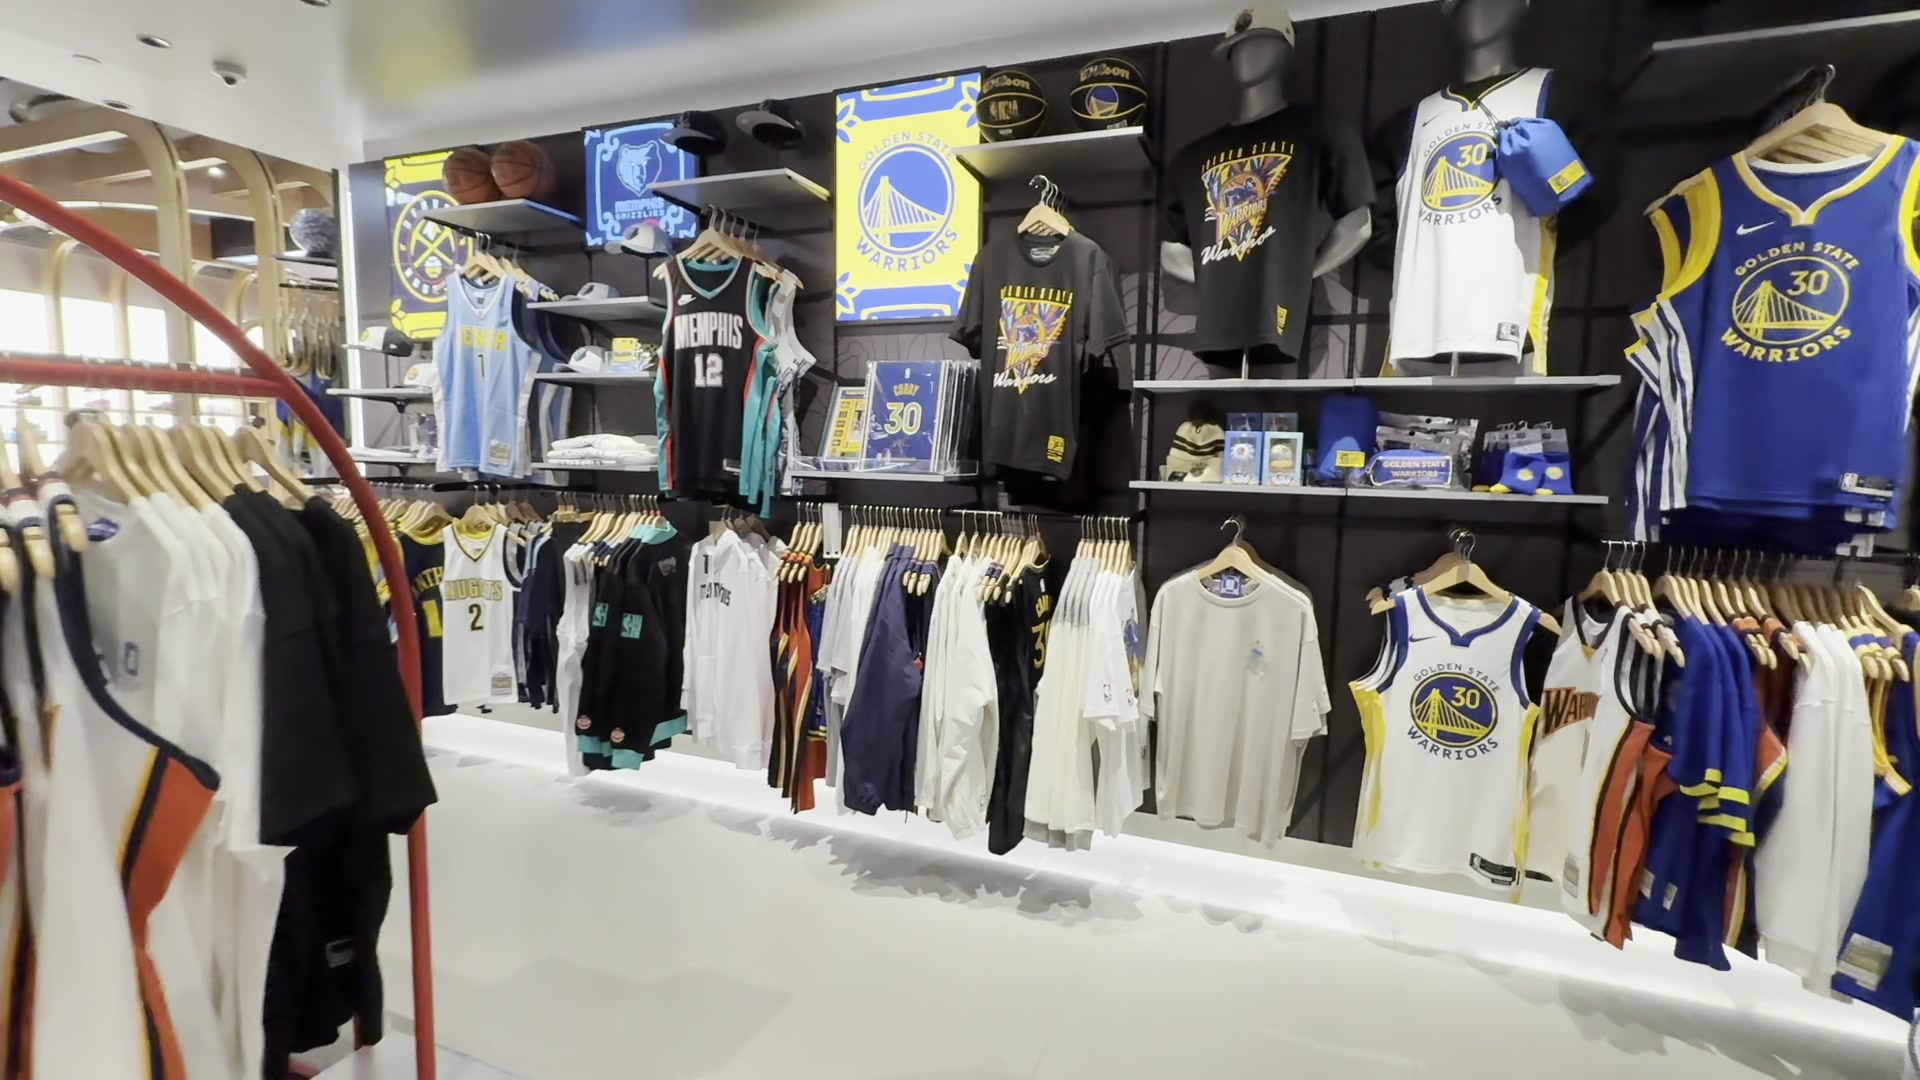
\includegraphics[width=0.82\linewidth]{fig10_nba_merchandise.jpg}
  \caption{NBA主题空间中的球衣与商品。全球体育文化首先以产品、球队标志和收藏品的形式出现。}
\end{figure}

\begin{figure}[H]
  \centering
  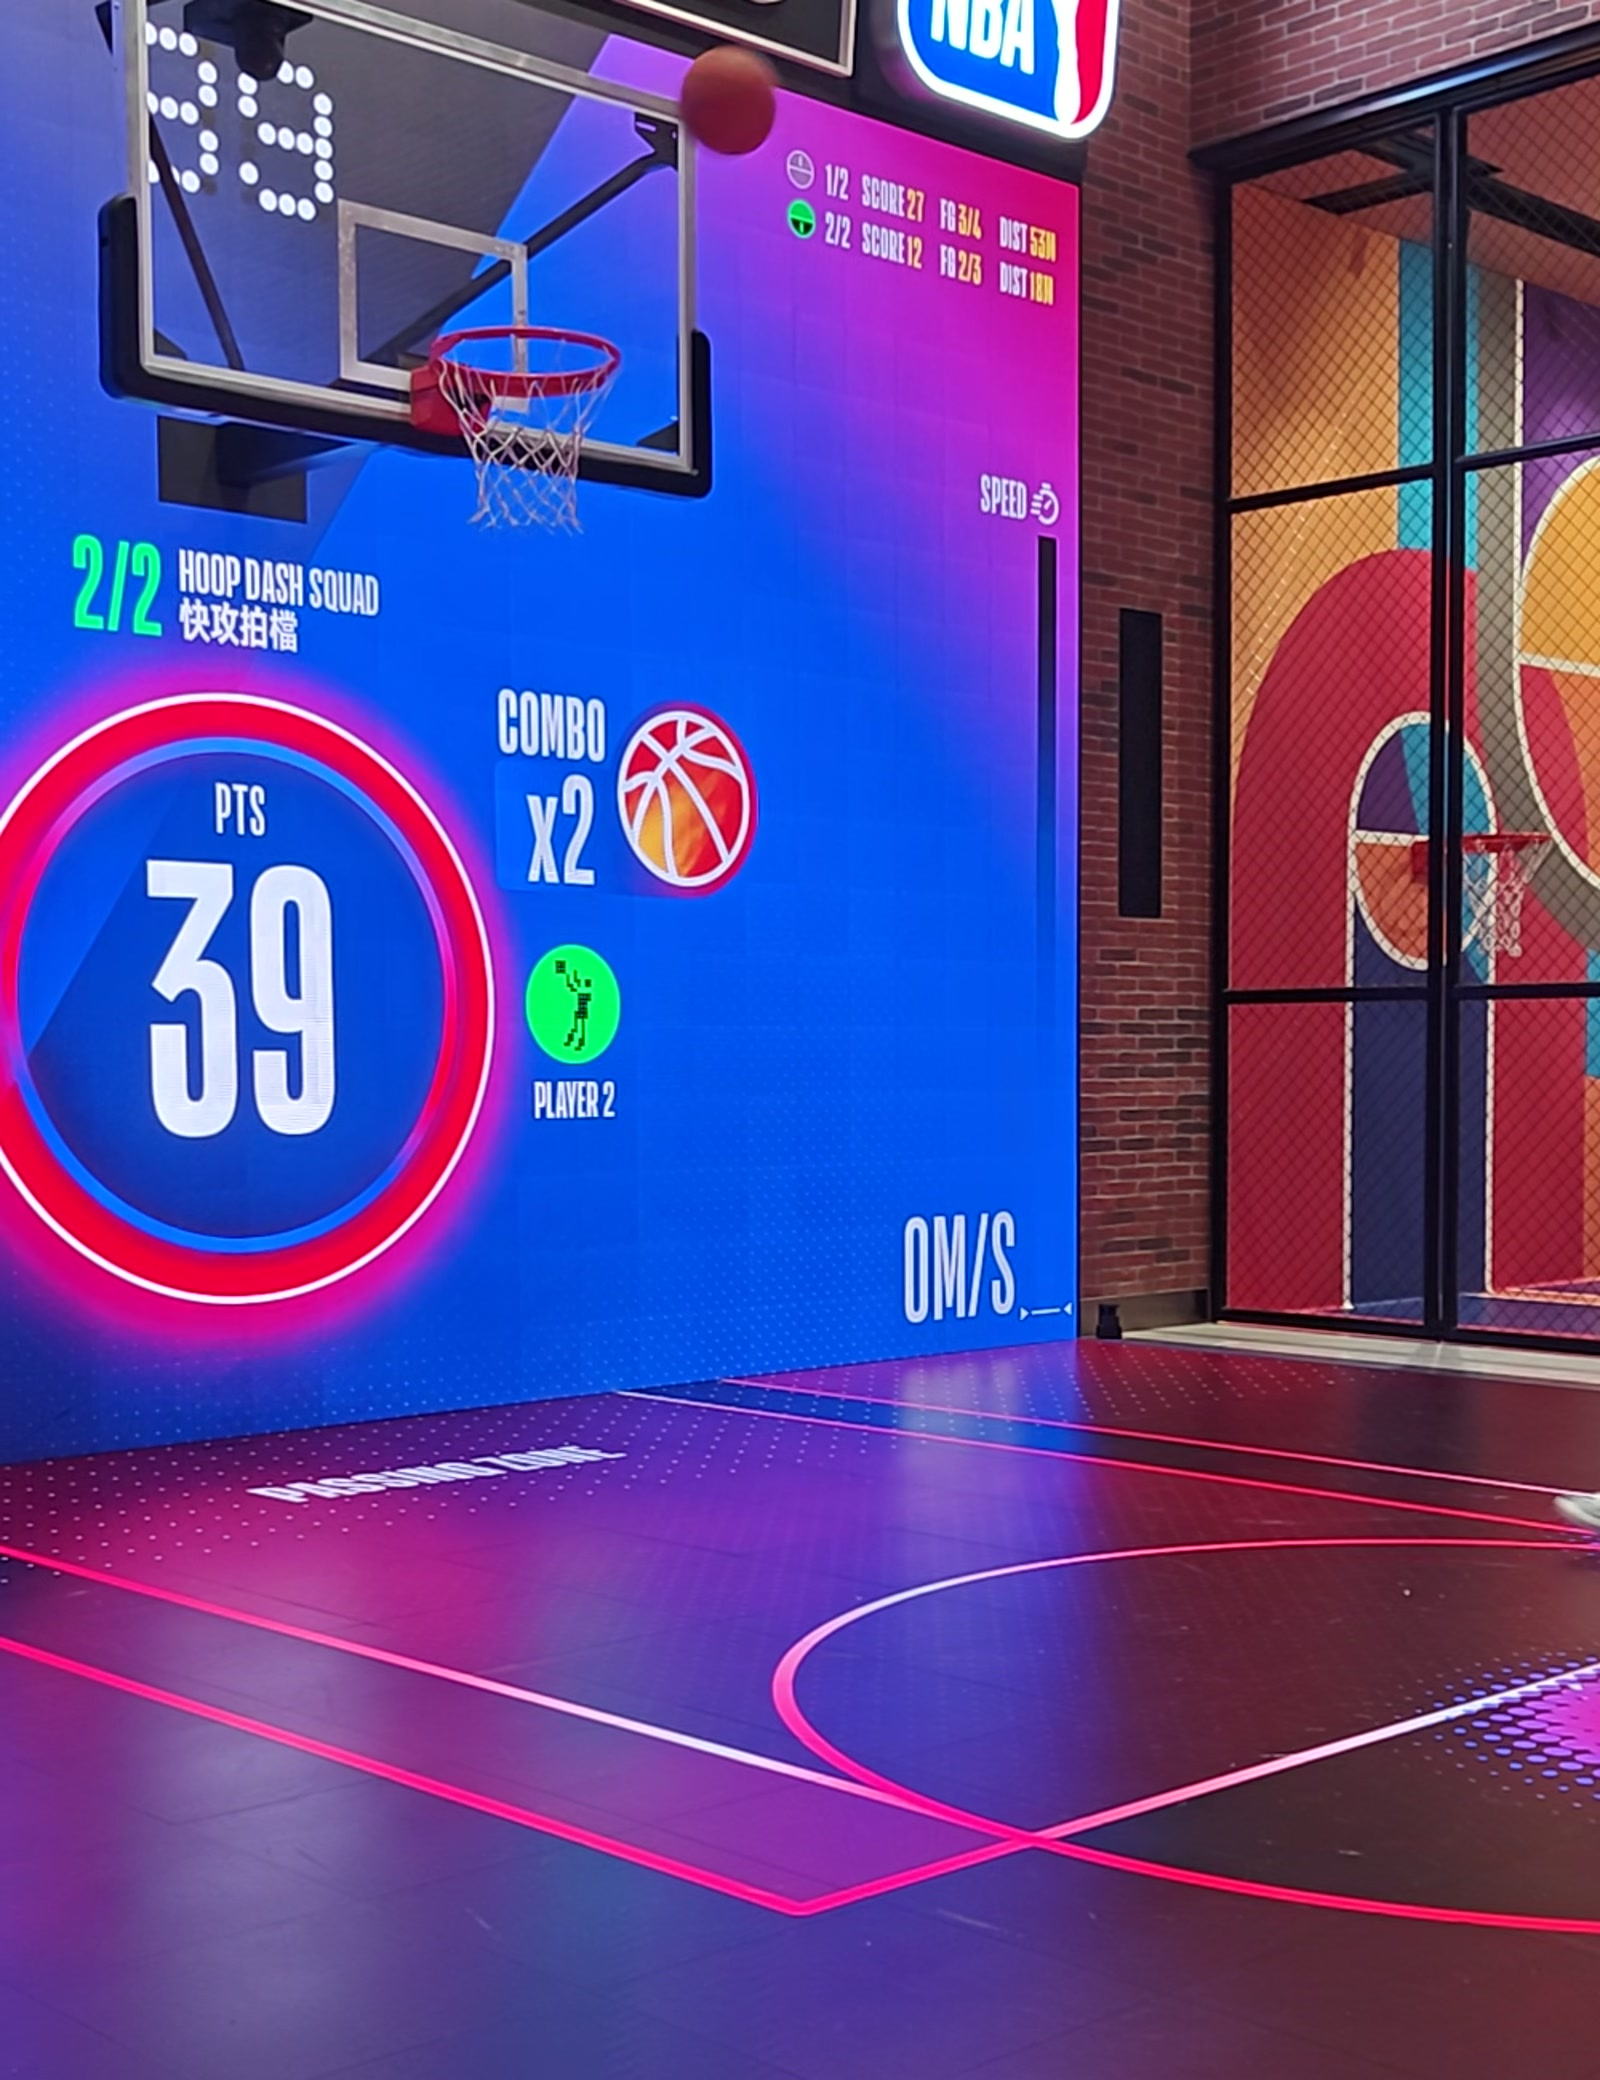
\includegraphics[width=0.82\linewidth]{fig7_nba.jpg}
  \caption{NBA投篮互动区域。篮筐、计分屏幕和投篮动作将体育文化转化为现场参与。}
\end{figure}

\subsection{交通澳门}

交通空间在田野报告中容易被忽略。巴士、穿梭车、桥梁、车窗和回程车厢看起来只是连接目的地，没什么别的。但它们也让不同版本的澳门一个接一个地出现。交通空间没有像遗产景点或主题酒店那样明确展示文化，而是在日常移动中展示了人群、节奏和城市层积。

\begin{figure}[H]
  \centering
  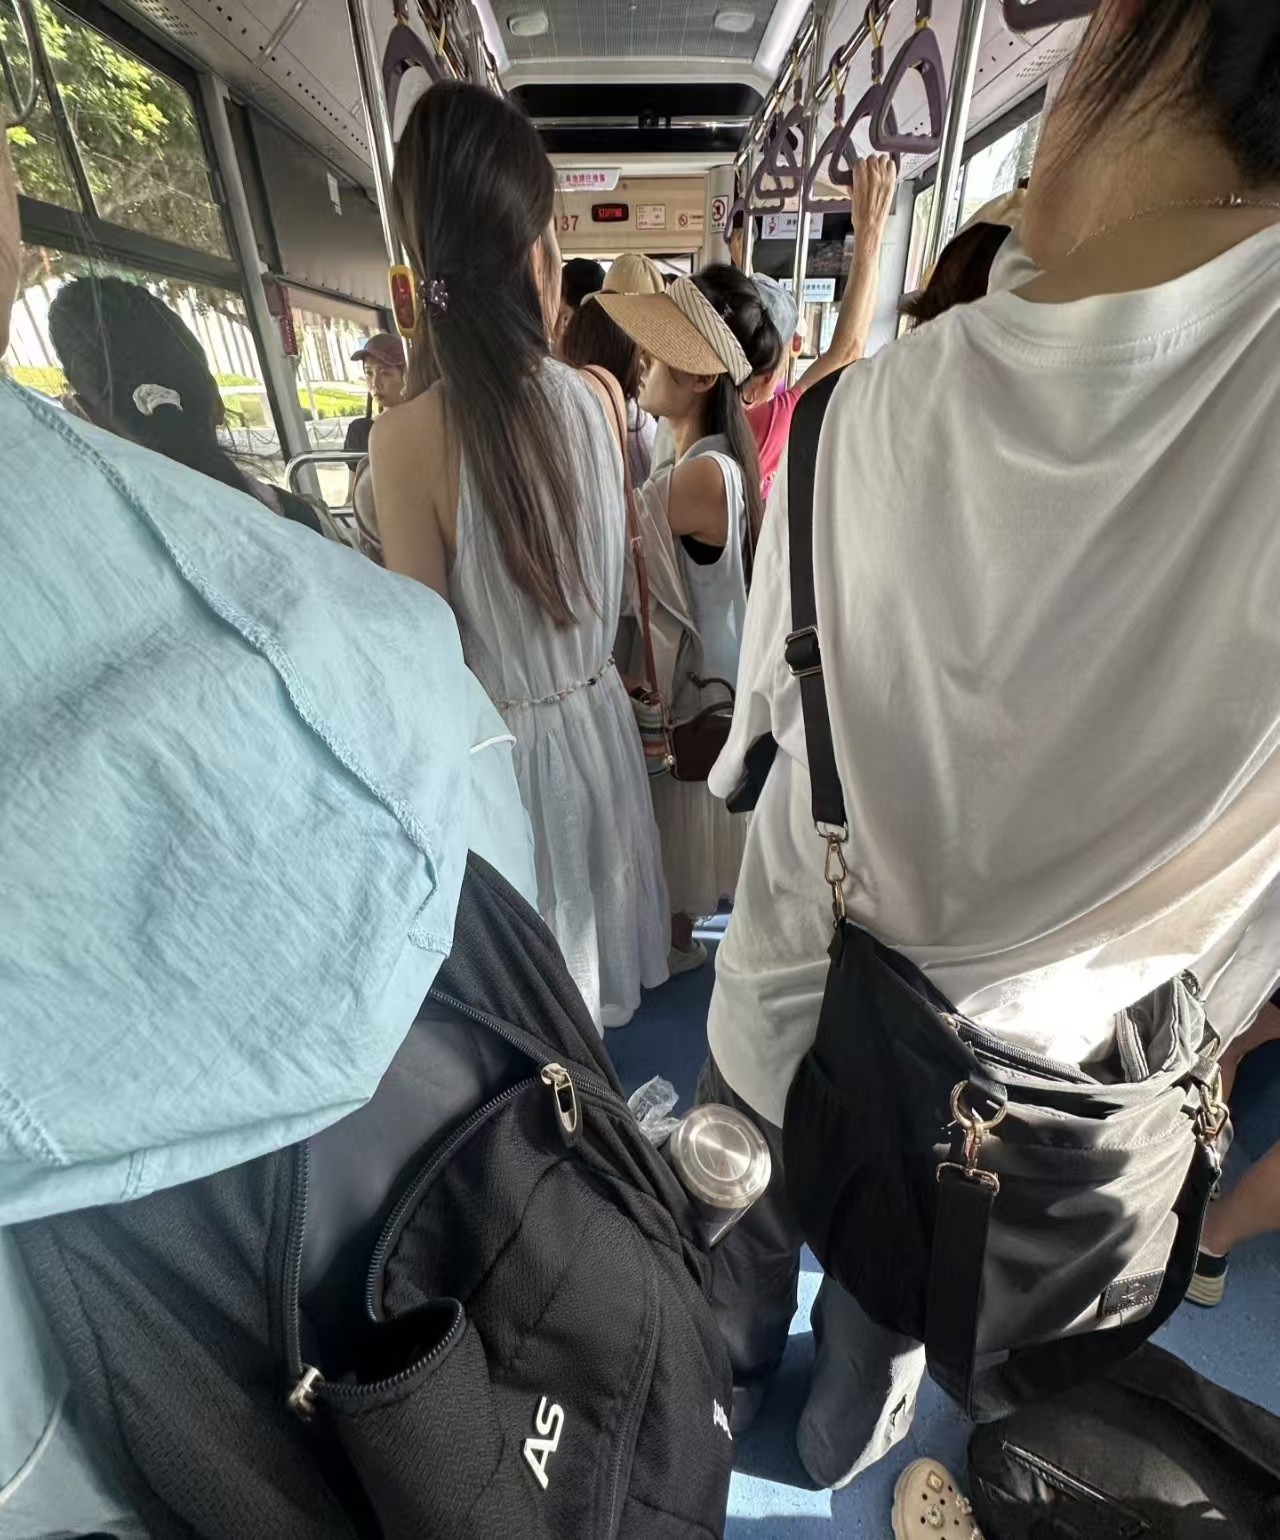
\includegraphics[width=0.82\linewidth]{fig10_bus_interior.jpg}
  \caption{拥挤的巴士内部。扶手、站立的身体和车辆密度展示了交通空间中的移动秩序。}
\end{figure}

\begin{figure}[H]
  \centering
  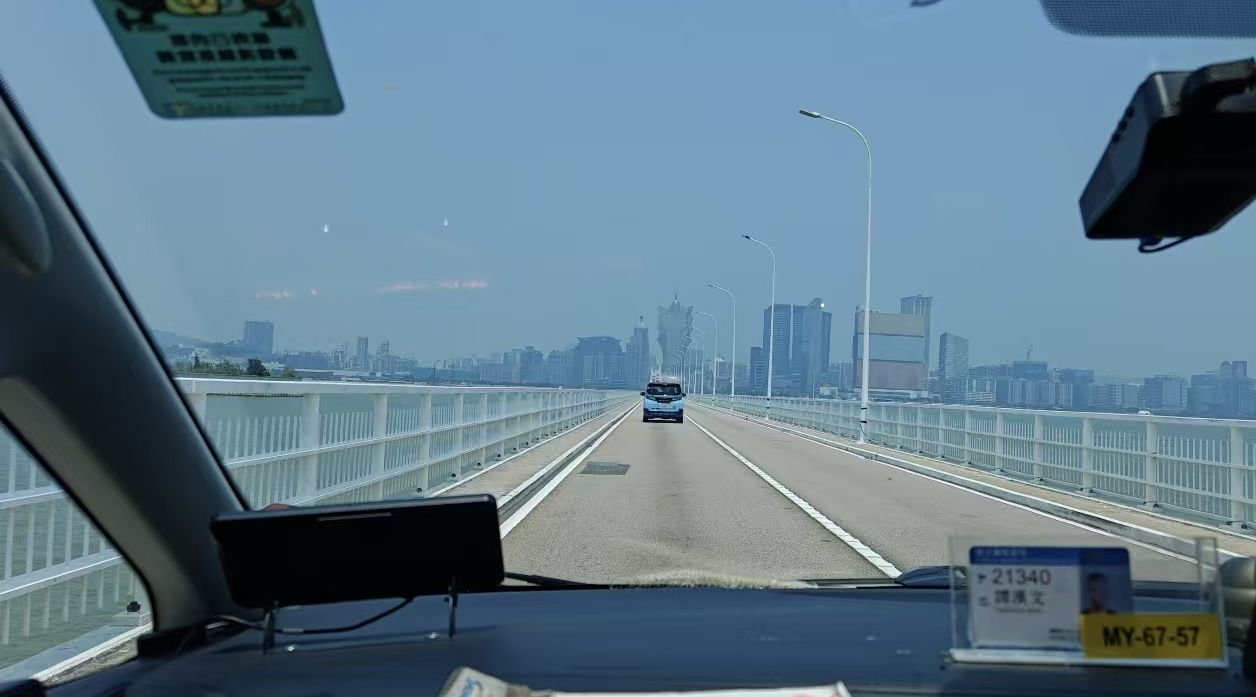
\includegraphics[width=0.82\linewidth]{fig12_vehicle_bridge.jpg}
  \caption{车内看到的桥梁移动。挡风玻璃、道路、桥梁和远处天际线将观察者限定在车窗视野中。}
\end{figure}

交通空间表明，澳门的跨文化体验不仅发生在目的地，也发生在目的地之间。de Certeau（1984）和Pink（2009）都提醒我们不要把移动当成空白时间。角色切换就在这些路线上发生。巴士车窗、桥梁、拥挤的座位——这些就是一个澳门让位给下一个澳门的地方。

\section{讨论}

\subsection{超越融合}

"中西融合"是理解澳门的合理起点，但作为最终解释不够。它能涵盖中葡历史、双语路名和葡式巷道。它应对不了商业街、路氹娱乐综合体、NBA主题空间和交通空间。当融合被用作唯一标签时，不同的文化元素被推进了同一个静态框架。

我们的路线指向另一种读法。澳门呈现为一系列空间转换，每一个都有自己的逻辑。口岸施加了边界和秩序。然后商业街把我们拉进消费，历史区域让我们放慢进入遗产观看，接着路氹把我们卷入全球娱乐，巴士又把我们带回日常城市移动。每一次转换都改变了我们如何行动和注意到什么。

这种读法并不否认澳门的中葡历史。正因为这段历史重要，它才需要被从其他文化体系中分离出来。文化敏感性不能停留在"多种文化并存"这一观察上。它需要追问：谁被引导进入这座城市，谁被邀请消费，谁被定位为历史观看者，谁通过互动参与全球娱乐。这些问题比"澳门是不是融合之城"更好地解释了我们的田野材料。

\subsection{路线改变了问题}

如果单独分析每个地点，澳门会碎裂为互不关联的旅游景点：口岸是交通，大三巴是遗产，商业街是消费，威尼斯人是娱乐，巴士是移动。一旦这些地点通过路线连接起来，问题就变了。地点之间的转换成为分析的一部分。

转换也改变了我们的位置。在口岸，制度程序管理着我们的进入。等走到美食街时，那些程序已被商业和人潮的拉力取代。后来，站在大三巴牌坊面前或威尼斯人内部，问题又变了——从买什么到看什么到怎么玩。回到巴士上，我们看着城市在车窗中重叠。

路线也提醒我们，我们并不是站在澳门之外给出一个中立的解释。我们被周围的系统反复定位。问题从澳门"是"什么文化，转变为人们在不同空间中如何被安排去体验文化。

\subsection{从标牌到身体}

跨文化沟通不止于语言翻译。中葡双语路牌和NBA英文界面塑造着地方身份，填充其间的非言语线索也同样如此。口岸走廊无需言语即可引导身体。大三巴的台阶和广场通过物理位置安排观看方式。威尼斯人的天花板和灯光不着一言便制造出沉浸感。NBA球场的篮筐和计分屏幕把文化变成了一场投篮游戏。甚至巴士车窗也在框定着什么能被看到、什么不能。

因此，本报告同时关注两个层面：一个空间说了什么，以及它对身体和行动做了什么。Landry和Bourhis（1997）帮助解释多语标牌如何塑造地方身份。Scollon和Scollon（2003）将标牌放回其具体位置。Hall（1959）提醒我们空间秩序本身就是一种非言语沟通。澳门的跨文化意义形成于书面标牌、身体秩序和感官体验之间。

\subsection{误读与诠释}

本报告的课程价值部分在于纠正几种可能的误读。简单地把澳门叫做中西融合之城，会遮蔽口岸、商业街、历史区和路氹之间的差异。把商业化视为对历史的削弱，忽略了商业街也通过味道和人群传播着遗产地标。把威尼斯人叫作"假欧洲"，忽视了它在澳门旅游经济中通过设计和参与生产体验的方式。还有一个限制：我们不能从拥挤的照片中推断居民或游客的主观态度，因为本研究没有包含正式访谈。

从文化相对主义的角度看，跨文化理解不应急于将一个空间标记为真实或不真实。更好的方法是追问它在自己的场景中如何运作、服务于谁、可能产生什么简化。当"融合"或"假欧洲"这样的快速解释不够用时，研究者必须回到具体的空间、路线和身体体验。这个修正过程本身就是反思性跨文化沟通的一部分。

\section{结论}

澳门的跨文化特征不会停留在某个地方不动。它随着路线移动。我们在边境作为被管理的对象进入，在美食街变成了买家，在旧石立面面前放慢成了观看者，然后在主题娱乐中重新加速为参与者，直到巴士把我们送回看着城市划过的位置。

中西融合在澳门是真实的。中葡文字、葡式建筑和世界遗产确实存在于街道上。但排队队伍、导视标牌、车窗、商品陈列、画出来的天幕和身体移动也在塑造文化体验，仅靠融合无法解释它们。

报告有局限。没有正式访谈，因此不能代表居民、游客或工人的主观声音。路线有限，无法覆盖澳门所有街区。声音和感官观察未通过系统音频研究收集，仅作为补充性田野笔记。未来研究可以加入居民和游客访谈、比较不同路线、或更系统地记录语言景观和交通空间。

对于跨文化沟通，这次田野考察给出了一个主要提醒：不要过快地给一座城市贴标签。进入具体空间，观察人们如何移动、观看、消费和参与，才能更审慎地理解文化在城市中如何被看见、使用和重新诠释。

\section*{参考文献}
\addcontentsline{toc}{section}{参考文献}

\noindent\hangindent=1.5em\hangafter=1
Chu, C. L. (2015). Spectacular Macau: Visioning futures for a World Heritage city. \textit{Geoforum, 65}, 440--450. \url{https://doi.org/10.1016/j.geoforum.2015.06.009}

\noindent\hangindent=1.5em\hangafter=1
Chung, T. (2009). Valuing heritage in Macau: On contexts and processes of urban conservation. \textit{Journal of Current Chinese Affairs, 38}(1), 129--160. \url{https://doi.org/10.1177/186810260903800107}

\noindent\hangindent=1.5em\hangafter=1
de Certeau, M. (1984). \textit{The practice of everyday life} (S. Rendall, Trans.). University of California Press.

\noindent\hangindent=1.5em\hangafter=1
Edensor, T. (2000). Staging tourism: Tourists as performers. \textit{Annals of Tourism Research, 27}(2), 322--344. \url{https://doi.org/10.1016/S0160-7383(99)00082-1}

\noindent\hangindent=1.5em\hangafter=1
Hall, E. T. (1959). \textit{The silent language}. Doubleday.

\noindent\hangindent=1.5em\hangafter=1
Landry, R., \& Bourhis, R. Y. (1997). Linguistic landscape and ethnolinguistic vitality: An empirical study. \textit{Journal of Language and Social Psychology, 16}(1), 23--49. \url{https://doi.org/10.1177/0261927X970161002}

\noindent\hangindent=1.5em\hangafter=1
Lefebvre, H. (1991). \textit{The production of space} (D. Nicholson-Smith, Trans.). Blackwell.

\noindent\hangindent=1.5em\hangafter=1
Ma, Q., \& Mu, C. (2023). Multilingual practices of translation in Macao's linguistic landscape: A case study of Rua do Campo. \textit{Cadernos de Tradução, 43}(1), 1--22. \url{https://doi.org/10.5007/2175-7968.2023.e90223}

\noindent\hangindent=1.5em\hangafter=1
MacCannell, D. (1973). Staged authenticity: Arrangements of social space in tourist settings. \textit{American Journal of Sociology, 79}(3), 589--603. \url{https://doi.org/10.1086/225585}

\noindent\hangindent=1.5em\hangafter=1
Pink, S. (2009). \textit{Doing sensory ethnography}. SAGE.

\noindent\hangindent=1.5em\hangafter=1
Scollon, R., \& Scollon, S. W. (2003). \textit{Discourses in place: Language in the material world}. Routledge.

\noindent\hangindent=1.5em\hangafter=1
UNESCO World Heritage Centre. (n.d.). \textit{Historic Centre of Macao}. Retrieved May 5, 2026, from \url{https://whc.unesco.org/en/list/1110/}

\noindent\hangindent=1.5em\hangafter=1
Urry, J., \& Larsen, J. (2011). \textit{The tourist gaze 3.0}. SAGE.

\noindent\hangindent=1.5em\hangafter=1
Wang, N. (1999). Rethinking authenticity in tourism experience. \textit{Annals of Tourism Research, 26}(2), 349--370. \url{https://doi.org/10.1016/S0160-7383(98)00103-0}

\noindent\hangindent=1.5em\hangafter=1
Yan, X. (2019). Language choices in the linguistic landscape of Macao. \textit{Journal of Multilingual and Multicultural Development, 40}(3), 198--217. \url{https://doi.org/10.1080/01434632.2018.1498853}

\appendix

\section{田野考察路线表}

\begin{table}[H]
\centering
\caption{田野考察路线、观察者角色与空间类型}
\begin{tabular}{>{\raggedright\arraybackslash}p{0.18\linewidth}>{\raggedright\arraybackslash}p{0.23\linewidth}>{\raggedright\arraybackslash}p{0.25\linewidth}>{\raggedright\arraybackslash}p{0.22\linewidth}}
\toprule
路线阶段 & 主要空间 & 观察者角色 & 主要机制 \\
\midrule
进入澳门 & 口岸、排队区、交通接驳 & 入境者 & 排队、导视、过关、车窗景观 \\
商业街道 & 美食街、纪念品街、标牌、人群 & 消费者 & 产品、语言景观、拥挤街道 \\
历史区域 & 大三巴牌坊、教堂空间、大炮台、路牌 & 观看者与阅读者 & 步行、摄影、双语标牌、俯瞰城市 \\
路氹奇观 & 威尼斯人、巴黎人、赌场空间、NBA主题空间 & 全球娱乐参与者 & 主题设计、导视、购物、互动游戏 \\
交通空间 & 巴士、桥梁、回程车辆 & 移动中的观察者 & 车窗、拥挤、重叠的城市层积 \\
\bottomrule
\end{tabular}
\end{table}

\section{精选媒体清单}

\begin{longtable}{>{\raggedright\arraybackslash}p{0.1\linewidth}>{\raggedright\arraybackslash}p{0.12\linewidth}>{\raggedright\arraybackslash}p{0.28\linewidth}>{\raggedright\arraybackslash}p{0.38\linewidth}}
\caption{精选图像及其分析功能}\\
\toprule
图号 & 文件 & 场景 & 分析功能 \\
\midrule
\endfirsthead
\toprule
图号 & 文件 & 场景 & 分析功能 \\
\midrule
\endhead
图1 & fig01 & 前往澳门的交通导视 & 展示跨文化体验从入境、标牌和移动开始。 \\
图2 & fig02 & 大三巴牌坊附近商业街人群 & 展示拥挤的街道如何改变遗产观看的节奏。 \\
图3 & fig03 & 街边烘焙店与小吃摊 & 展示品尝、购买和停留如何成为身体体验。 \\
图4 & fig04 & 通往大三巴牌坊的街道 & 展示遗产观看如何被街道移动和商业塑造。 \\
图5 & fig05 & 蓝白瓷砖路牌 & 展示双语路牌如何保存城市记忆。 \\
图6 & fig06 & ``馬統領街''路牌 & 展示路名如何在日常空间中成为历史文本。 \\
图7 & fig07 & 通往大炮台的入口路径 & 展示遗产如何成为步行体验。 \\
图8 & fig08 & 路氹车窗景观 & 展示主题建筑如何进入城市想象。 \\
图9 & fig09 & 威尼斯人室内穹顶 & 展示欧洲意象如何被设计为沉浸体验。 \\
图10 & fig10 & 赌场与酒店导视 & 展示导视系统如何组织路氹的消费路线。 \\
图11 & fig11 & NBA商品展示 & 展示全球体育文化如何成为商品。 \\
图12 & fig12 & NBA投篮互动区域 & 展示体育文化如何成为参与式娱乐。 \\
图13 & fig13 & 巴士内部 & 展示交通空间中的移动秩序。 \\
图14 & fig14 & 车内桥梁景观 & 展示车窗如何在运动中框定澳门。 \\
\bottomrule
\end{longtable}

\section{课程ILO与评分标准对照}

\begin{table}[H]
\small
\centering
\caption{课程ILO与报告内容对照}
\begin{tabular}{>{\raggedright\arraybackslash}p{0.14\linewidth}>{\raggedright\arraybackslash}p{0.42\linewidth}>{\raggedright\arraybackslash}p{0.32\linewidth}}
\toprule
课程目标 & 报告对照 & 主要章节 \\
\midrule
ILO\#1 & 路线进入与角色切换展示了观察者与他者之间的空间关系 & 引言、发现、讨论5.2 \\
ILO\#2 & 报告避免将澳门简化为单一融合标签，区分了不同文化逻辑 & 引言、讨论5.1 \\
ILO\#3 & 报告分析了路牌、店招、导视、排队、车窗和互动设施中的言语与非言语沟通 & 框架、发现、讨论5.3 \\
ILO\#4 & 路线被用于构建文化敏感的田野叙事，而非旅游景点清单 & 方法、讨论5.2 \\
ILO\#5 & 报告识别并纠正了"假欧洲"和"商业化削弱历史"等诠释性误读 & 讨论5.4、结论 \\
\bottomrule
\end{tabular}
\end{table}

\end{document}
